% Fig. 1 "SMOLDER in brief" -- standalone TikZ version (full text width, 17.7 cm).
% Compile with pdflatex next to fig1_risk_thumbnail.png. To use it inside the paper,
% copy the tikzpicture environment (and the colour/size definitions) into the .tex file.
\documentclass[tikz,border=1pt]{standalone}
\usepackage[scaled=0.92]{helvet}   % Helvetica, like the other figures of the paper
\renewcommand{\familydefault}{\sfdefault}
\usepackage{graphicx}
\usetikzlibrary{arrows.meta}

\definecolor{ink}{HTML}{222222}
\definecolor{greytxt}{HTML}{6E6E6E}
\definecolor{slow}{HTML}{3A6B9A}  \definecolor{slowbg}{HTML}{E3EBF4}
\definecolor{fast}{HTML}{A8682A}  \definecolor{fastbg}{HTML}{F4E9DC}
\definecolor{tgt}{HTML}{9B2F2F}   \definecolor{tgtbg}{HTML}{F4E1E1}
\definecolor{neut}{HTML}{EEEEEE}
\newcommand{\sz}[2]{\fontsize{#1}{#2}\selectfont}

\begin{document}
\begin{tikzpicture}[x=0.177cm, y=0.177cm, line join=miter, line cap=butt,
    >={Stealth[length=3.2pt, width=2.6pt]},
    lab/.style={inner sep=0pt, font=\sz{6.6}{7.9}},
    body/.style={inner sep=0pt, align=center, font=\sz{6.3}{7.3}},
    head/.style={inner sep=0pt, font=\sz{6.9}{8.2}\bfseries},
    group/.style={draw=greytxt, line width=0.6pt, dash pattern=on 3pt off 2pt},
    cell/.style={line width=0.8pt}]

% ------------------------------------------------------------ (a) input windows and target
\node[anchor=west, inner sep=0pt, font=\sz{7.6}{9}\bfseries] at (0.8,36.6) {(a) What the model reads, and what it forecasts};
\node[anchor=east, inner sep=0pt, font=\sz{6}{7}\itshape, text=greytxt] at (99.2,36.6) {not to scale};

\draw[ink, line width=0.7pt, ->] (2.5,25.7) -- (98.8,25.7);
\foreach \x in {6,52,74,92} \draw[ink, line width=0.7pt] (\x,25.1) -- (\x,26.3);
\node[lab] at (6,23.8)  {\textit{D}\,\textminus\,144 days};
\node[lab] at (52,23.8) {\textit{D}\,\textminus\,14 days};
\node[lab] at (74,23.8) {issue day \textit{D}};
\node[lab] at (92,23.8) {\textit{D}\,+\,3};
\node[lab, anchor=east, text=greytxt] at (98.8,23.8) {time};

% slow window, 18 eight-day steps
\draw[slow, fill=slowbg, line width=0.8pt] (6,31.4) rectangle (74,34.9);
\foreach \k in {1,...,17} \draw[slow, line width=0.5pt] ({6+\k*68/18},31.4) -- ++(0,0.7);
\node[lab, text=slow] at (40,33.4) {Slow branch: 18 eight-day means of leaf area index, soil moisture and rain\enspace$\rightarrow$\enspace fuel amount and dryness};

% fast window, 14 daily steps
\draw[fast, fill=fastbg, line width=0.8pt] (52,27.5) rectangle (74,30.8);
\foreach \k in {1,...,13} \draw[fast, line width=0.5pt] ({52+\k*22/14},27.5) -- ++(0,0.7);
\node[lab, text=fast] at (63,29.3) {Fast branch: 14 daily maps};
\node[lab, text=fast, anchor=east] at (51,29.15) {weather, greenness, recent fire\enspace$\rightarrow$\enspace current conditions};

% forecast target
\draw[tgt, fill=tgtbg, line width=0.8pt] (74.5,27.5) rectangle (92,34.9);
\node[head, text=tgt] at (83.25,33.1) {Target};
\node[body, text=tgt] at (83.25,30.1) {fire detected on\\day \textit{D}+1, \textit{D}+2 or \textit{D}+3?};

% ------------------------------------------------------------ (b) processing pipeline
\node[anchor=west, inner sep=0pt, font=\sz{7.6}{9}\bfseries] at (0.8,21.4) {(b) How the information is processed};
\draw[group] (0.8,0.5)  rectangle (23.2,20.0);
\draw[group] (25.4,0.5) rectangle (55.6,20.0);
\draw[group] (57.8,0.5) rectangle (99.2,20.0);
\node[anchor=west, inner sep=0pt, font=\sz{7.4}{8.8}\bfseries] at (1.7,18.6)  {1};
\node[anchor=west, inner sep=0pt, font=\sz{6.8}{8.1}, text=greytxt] at (3.4,18.6)  {Inputs};
\node[anchor=west, inner sep=0pt, font=\sz{7.4}{8.8}\bfseries] at (26.3,18.6) {2};
\node[anchor=west, inner sep=0pt, font=\sz{6.8}{8.1}, text=greytxt] at (28.0,18.6) {Encoders (ConvLSTM)};
\node[anchor=west, inner sep=0pt, font=\sz{7.4}{8.8}\bfseries] at (58.7,18.6) {3};
\node[anchor=west, inner sep=0pt, font=\sz{6.8}{8.1}, text=greytxt] at (60.4,18.6) {Fusion and output};

% group 1: inputs
\draw[slow, fill=slowbg, line width=0.8pt] (1.8,10.0) rectangle (22.2,17.0);
\node[head, text=slow] at (12,15.4) {Fuel and moisture};
\node[body] at (12,12.3) {leaf area index,\\soil moisture, rain};
\draw[fast, fill=fastbg, line width=0.8pt] (1.8,1.4) rectangle (22.2,8.4);
\node[head, text=fast] at (12,6.8) {Weather and fire};
\node[body] at (12,3.7) {heat, dry air (VPD), wind, NDVI,\\recent fire, fire intensity, fuel age};

% group 2: encoders as chains of ConvLSTM cells (slow row centre y = 12.5, fast row centre y = 3.9)
\foreach \yc/\col/\bg in {11.1/slow/slowbg, 2.5/fast/fastbg} {
  \foreach \x in {27.4,32.5,37.6,47.8} \draw[\col, fill=\bg, cell] (\x,\yc) rectangle ++(3.2,2.8);
  \node[lab, text=\col] at (44.3,\yc+1.4) {$\cdots$};
  \draw[\col, line width=0.7pt, ->] (30.6,\yc+1.4) -- (32.5,\yc+1.4);
  \draw[\col, line width=0.7pt, ->] (35.7,\yc+1.4) -- (37.6,\yc+1.4);
  \draw[\col, line width=0.7pt, ->] (40.8,\yc+1.4) -- (43.2,\yc+1.4);
  \draw[\col, line width=0.7pt, ->] (45.4,\yc+1.4) -- (47.8,\yc+1.4);
}
\node[head, text=slow, anchor=west] at (27.4,15.6) {Slow memory};
\node[lab, text=greytxt, anchor=east, font=\sz{6.2}{7.4}] at (51.0,15.6) {18 steps};
\node[head, text=fast, anchor=west] at (27.4,7.0)  {Fast memory};
\node[lab, text=greytxt, anchor=east, font=\sz{6.2}{7.4}] at (51.0,7.0)  {14 steps};
\draw[slow, line width=0.8pt, ->] (22.2,12.5) -- (27.4,12.5);
\draw[fast, line width=0.8pt, ->] (22.2,3.9)  -- (27.4,3.9);

% group 3: combine, risk map, flag
\draw[ink, fill=neut, line width=0.8pt] (59,2.0) rectangle (67.6,16.4);
\node[head] at (63.3,11.4) {Combine};
\node[body, font=\sz{6.1}{7.1}] at (63.3,7.6) {slow summary\\added to each\\fast step};
\draw[slow, line width=0.8pt, ->] (51.0,12.5) -- (59,12.5);
\draw[fast, line width=0.8pt, ->] (51.0,3.9)  -- (59,3.9);

\node[anchor=south west, inner sep=0pt] at (70.6,3.1) {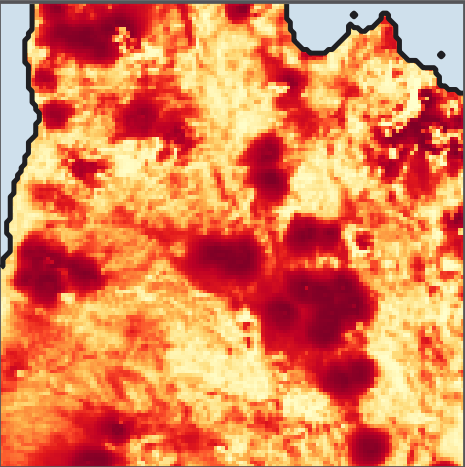
\includegraphics[width=1.947cm, height=1.947cm]{fig1_risk_thumbnail.png}};
\draw[ink, line width=0.7pt] (70.6,3.1) rectangle (81.6,14.1);
\node[lab, font=\sz{6.4}{7.6}\bfseries] at (76.1,15.3) {Risk score per 1\,km pixel};
\node[lab, font=\sz{5.8}{7}, text=greytxt] at (76.1,2.1) {darker = higher risk};
\draw[ink, line width=0.8pt, ->] (67.6,9.2) -- (70.6,9.2);

\draw[tgt, fill=tgtbg, line width=0.8pt] (85,4.2) rectangle (98.2,14.2);
\node[head, text=tgt] at (91.6,11.4) {Flag};
\node[body, font=\sz{6.1}{7.1}] at (91.6,7.6) {pixels above one\\fixed threshold\\(chosen on 2019)};
\draw[ink, line width=0.8pt, ->] (81.6,9.2) -- (85,9.2);
\end{tikzpicture}
\end{document}
